\section{Semantic Search in the Engine}
\label{sec-sem}\label{sec-order}\label{sec-vectors}\label{sec-hybrid}

\stitle{Order is not similarity}.
A sorted index answers a bound prefix with one range scan, and it is tempting
to hope that terms close in meaning are close in the order.
\begin{lemma}[Bandwidth]\label{lem-bw}
Let $G$ be a graph with $N$ vertices and diameter $D$.
In every linear order of the vertices some edge joins vertices at least
$(N-1)/D$ positions apart.
\end{lemma}
For the neighbor graph of a $d$-dimensional grid of $N=g^d$ points this is at
least $g^{d-1}/d$ positions, so a scan of width $w$ cannot contain all
neighbors unless $w$ is that large.
On the Gene Ontology ($N=38{,}092$ terms, 384-dimensional embeddings of the names
by \texttt{all-MiniLM-L6-v2}~\cite{reimers2019}) the best order we tried, the
postorder of the class hierarchy, finds only 38\% of a term's ten nearest
neighbors within 100 positions, and \sys's first-seen ids 21\%.
The order serves structure, not similarity, so \sys adds vector indexes.

\begin{table}[t]
\caption{Share of the 10 nearest neighbors (by cosine) found within $\pm W$ positions of a term, and the median position gap to the nearest neighbor. GO, 38,092 terms, 2,000 queries.}
\label{tab-order}
\small
\resizebox{\columnwidth}{!}{%
\begin{tabular}{@{}lrrrrrr@{}}
\toprule
Order & gap & $\pm$50 & $\pm$100 & $\pm$500 & $\pm$1000 & $\pm$5000 \\
\midrule
dictionary id (first seen) & 1739 & .195 & .211 & .258 & .284 & .438 \\
hierarchy, deepest parent & 45 & .328 & .377 & .498 & .561 & .735 \\
hierarchy, first parent & 37 & .319 & .366 & .481 & .546 & .726 \\
label, alphabetical & 1749 & .310 & .334 & .379 & .408 & .558 \\
random & 10823 & .003 & .005 & .024 & .049 & .242 \\
\bottomrule
\end{tabular}}
\end{table}


\begin{figure}[t]
\centering
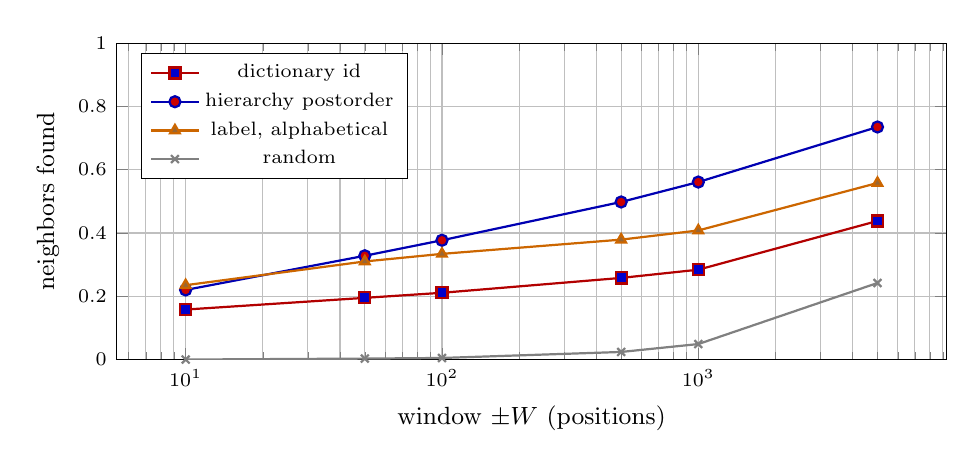
\begin{tikzpicture}
\begin{axis}[width=\columnwidth,height=5.6cm,xmode=log,xlabel={window $\pm W$ (positions)},ylabel={neighbors found},ymin=0,ymax=1,grid=both,legend pos=north west,legend style={font=\scriptsize},tick label style={font=\scriptsize},label style={font=\small}]
\addplot+[mark=square*,color=red!70!black,thick] coordinates {(10,0.158) (50,0.195) (100,0.211) (500,0.258) (1000,0.284) (5000,0.438)};
\addlegendentry{dictionary id}
\addplot+[mark=*,color=blue!70!black,thick] coordinates {(10,0.22) (50,0.328) (100,0.377) (500,0.498) (1000,0.561) (5000,0.735)};
\addlegendentry{hierarchy postorder}
\addplot+[mark=triangle*,color=orange!80!black,thick] coordinates {(10,0.235) (50,0.31) (100,0.334) (500,0.379) (1000,0.408) (5000,0.558)};
\addlegendentry{label, alphabetical}
\addplot+[mark=x,color=gray,thick] coordinates {(10,0) (50,0.003) (100,0.005) (500,0.024) (1000,0.049) (5000,0.242)};
\addlegendentry{random}
\end{axis}
\end{tikzpicture}

\caption{The data of Table~\ref{tab-order}: the share of neighbors found within $\pm W$ positions, by order.}
\label{fig-order}
\end{figure}


\stitle{Vector indexes in the engine}.
One unit vector $\mathbf{v}(t)$ per term is held in memory, and four index
families are available: exact (flat) search, IVF~\cite{jegou2011}, product
quantization (PQ), and HNSW~\cite{malkov2020}.
IVF clusters the vectors into $\nu$ lists and reads the $\rho$ nearest; its
lists are stored \emph{as key ranges of the B+ tree that holds the triples}, the
key $(\mathrm{list},\mathrm{row},0)$, so a list is a prefix scan and lists
page, cache, latch, and update like every other index of the engine.

\stitle{Filtering by a class}.
A filtered query $\mathrm{near}(q,c,k)$ asks for the $k$ terms of $\desc(c)$
nearest to $q$.
\emph{Pre-filter} resolves $c$ by interval scans and scores its members
exactly; \emph{post-filter} asks an index for more than $k$ and keeps those
below $c$ (a binary search over $I(c)$); \emph{masked search} gives the index
the predicate ``the row's label lies in an interval of $I(c)$'', so nothing is
resolved in advance.
\emph{Auto} pre-filters when $|\desc(c)|\le 4{,}096$ and otherwise masks HNSW.
The filter is \emph{correlated} with the vectors: the names of a class's
descendants are close to one another, so of the top 100 neighbors of a query from
\emph{inside} $c$, 4\% to 72\% lie under $c$, and from \emph{outside} only 0\% to
12\%.
The independence estimate $k/f(c)$ of the candidates needed, with
$f(c)=|\desc(c)|/N$, is wrong in both directions: post-filtering is cheap for an
inside query and fails for an outside one.
Testing membership with $I(c)$ per row touched, with no scan, makes masked
search 6 times faster than resolving the filter first.
